\subsubsection{GPS-Qualität}
\label{sec:gps_accuracy_definition}

\paragraph{[FR4]} Wenn die Genauigkeit der Positionierung unzuverlässig ist, muss \textit{NUNAV Navigation} den \textit{End Usern} anzeigen, dass die Positionierung aktuell nicht zuverlässig ist.

Die letzte entwickelte Erklärung betrifft den Aspekt der \textit{Scrutability}. Ziel ist es \textit{End Usern} anzuzeigen, wenn sie sich aktuell auf die Position auf der Route nicht verlassen können. Dies ist zum Beispiel in Tunneln der Fall und besonders kritisch, wenn in Kürze ein Abbiege-Kommando erfolgt und somit an der falschen Stelle kommt. Bewusst wurde auf die technische Bezeichnung \glqq GPS\grqq{} verzichtet.

\begin{figure}[htb!]
    \centering
    \subfloat[Prototyp zum Design bei schlechtem GPS]
    {
        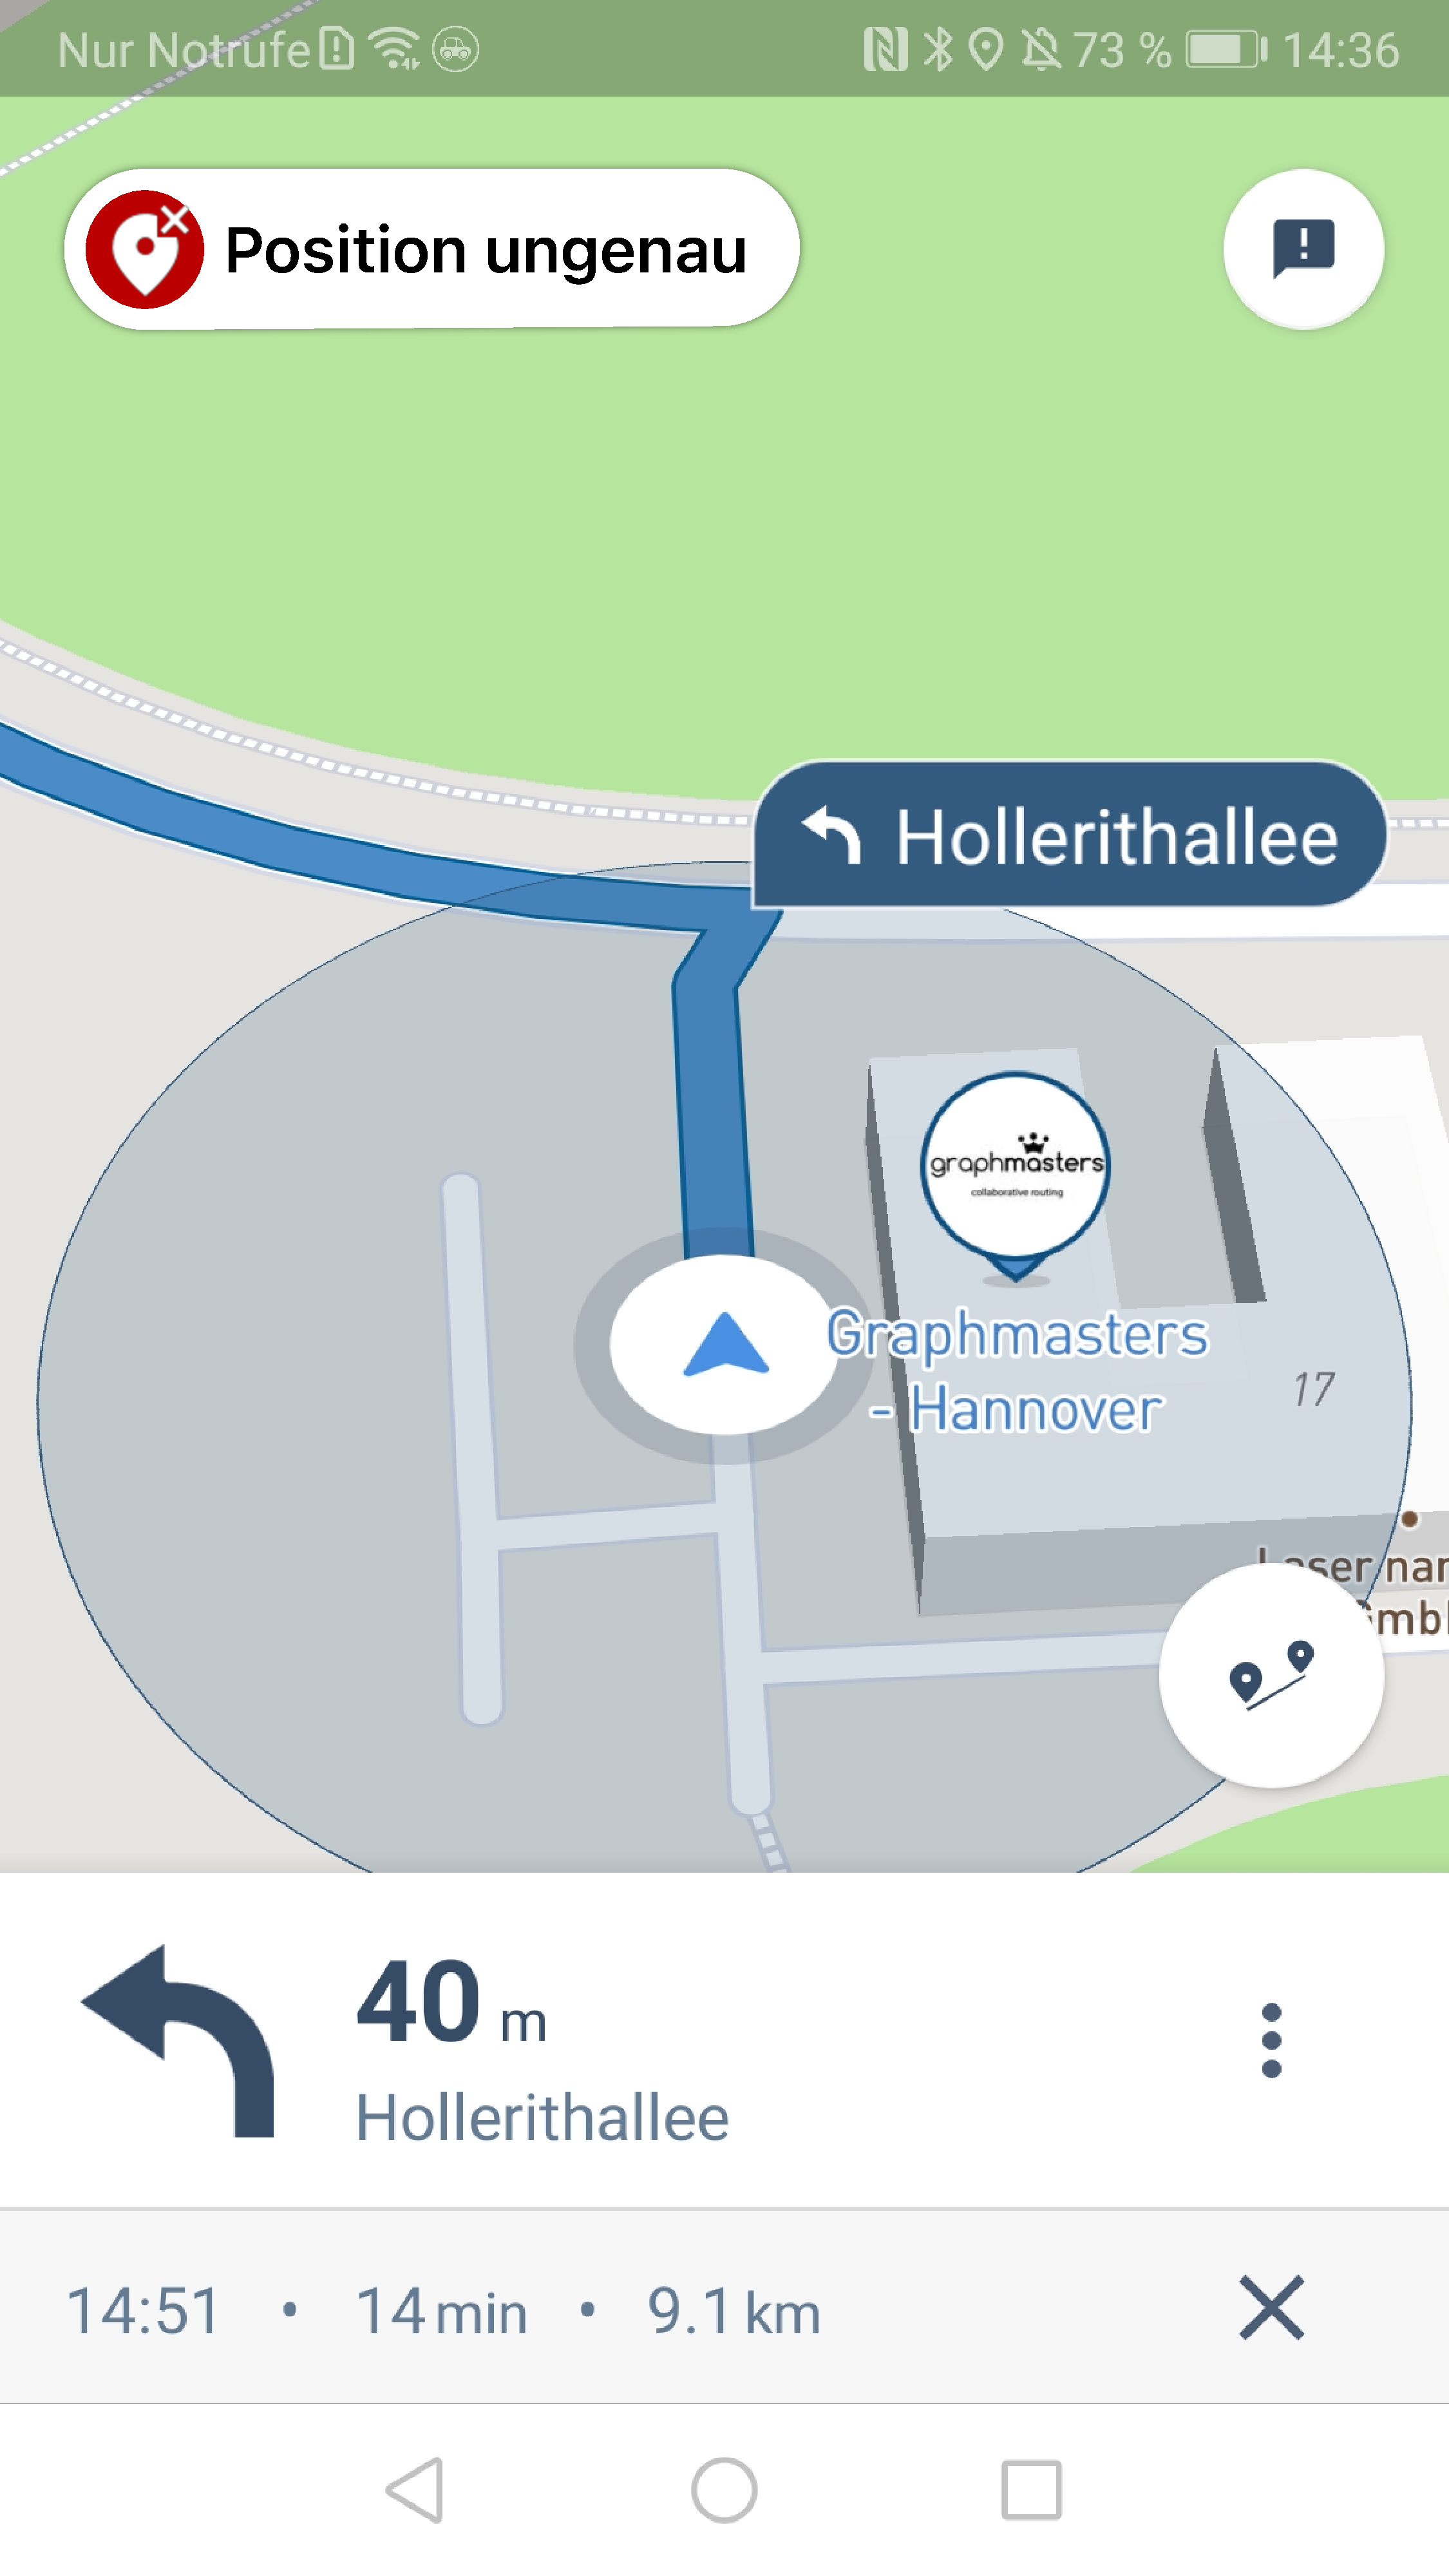
\includegraphics[width=.27\linewidth]{contents/06_model_evaluation/01_integration/res/04_position_accuracy/prototype_1.pdf}
    }
    \hspace{.055\linewidth}
    \subfloat[Finales Design bei schlechtem GPS]
    {
        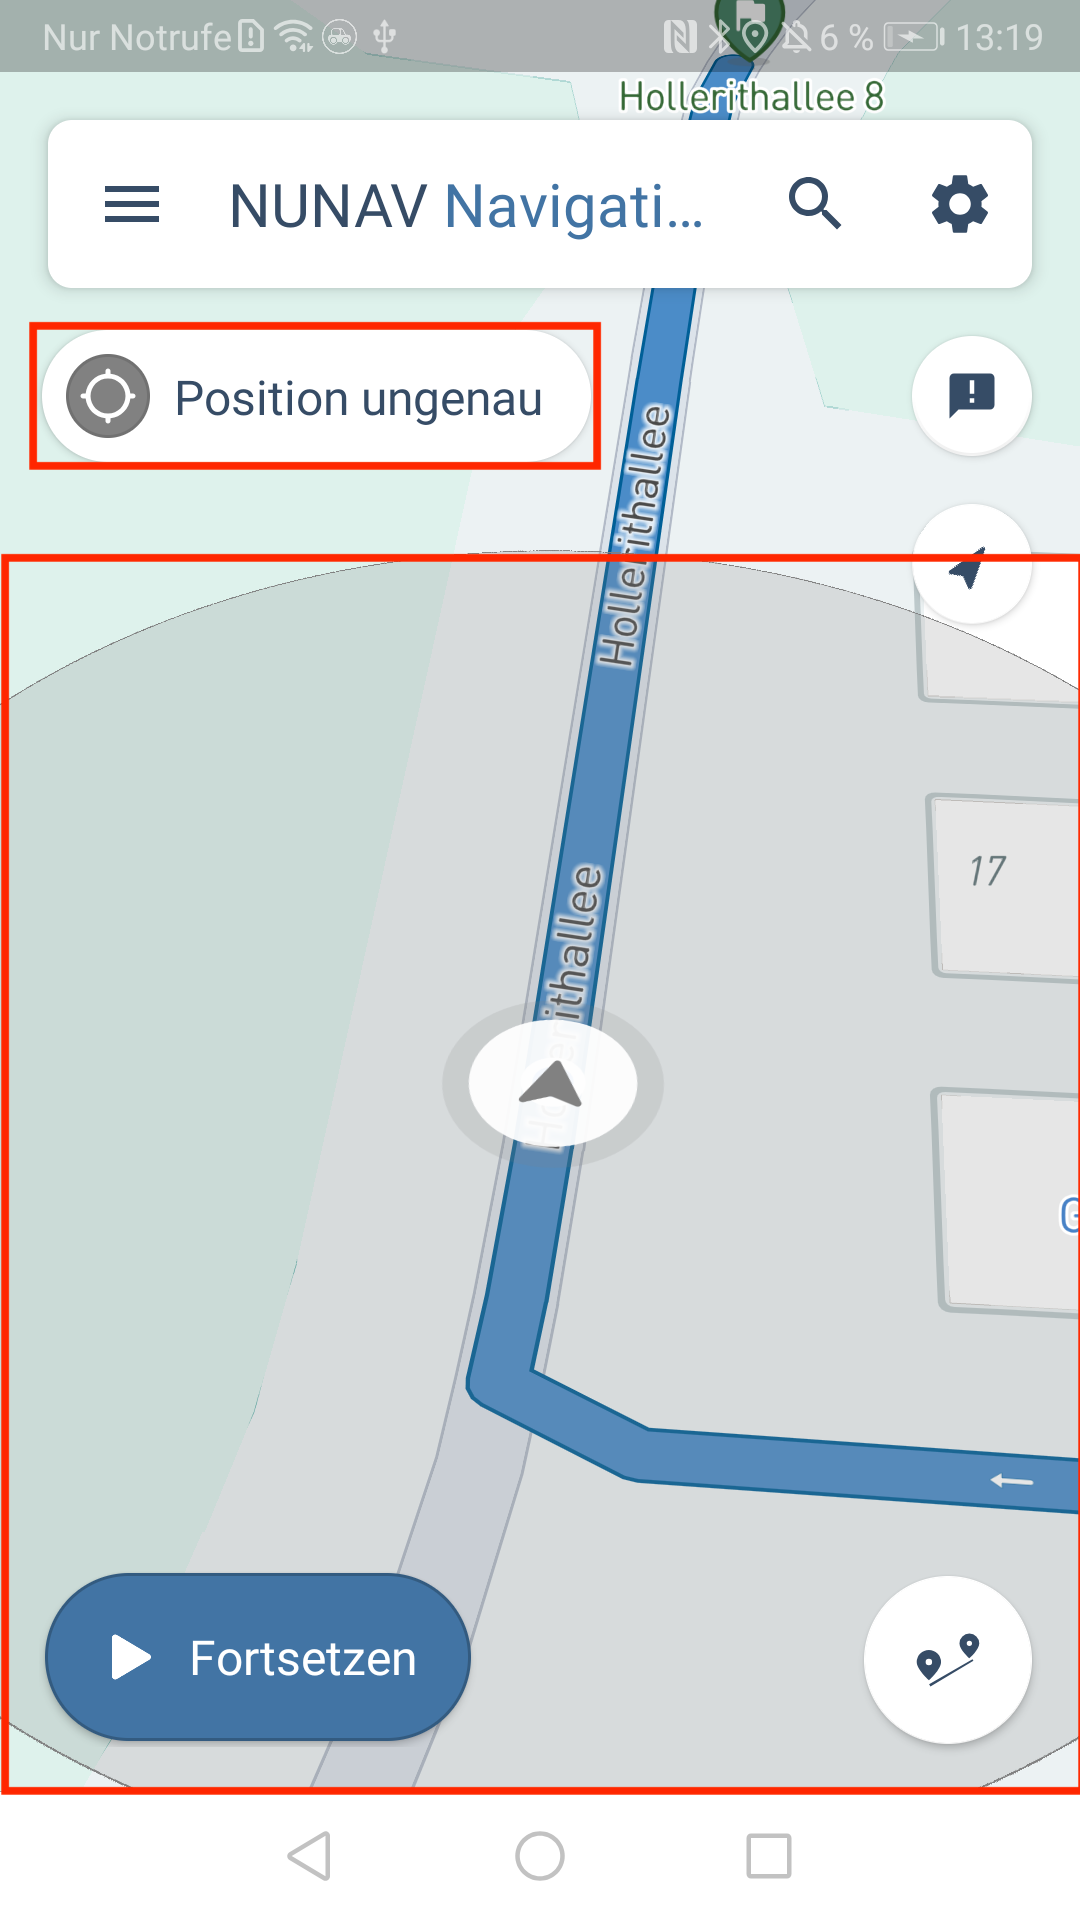
\includegraphics[width=.27\linewidth]{contents/06_model_evaluation/01_integration/res/04_position_accuracy/final_1.png}
    }
    \caption{Prototyp und finales Design für die Anzeige von schlechtem GPS während der Navigation}
    \label{fig:prototype_position_accuracy}
\end{figure}

Für die Entscheidung, wann das GPS ungenau ist, wurde innerhalb der \textit{NUNAV Navigation}-App ein neuer Algorithmus integriert, der diese trifft. Dabei spielt nicht nur die Genauigkeit, welche durch das GPS-Modul des Gerätes ermittelt wird, eine Rolle, sondern auch die Zeit, wann das letzte GPS-Update kam, da bei sehr schlechtem GPS keine Positionsupdates mehr vom Gerät geliefert werden. Der Algorithmus ist in den Zusatzmaterialien zu finden.

Als Design wurde im ersten Entwurf lediglich ein \textit{Growl} angezeigt und die Sprachansage \glqq Position ungenau\grqq{} ausgegeben. Insbesondere, wenn zum gleichen Zeitpunkt weitere \textit{Growls} angezeigt werden und die Sprachansagen vom \textit{End User} generell deaktiviert sind, hat sich die Sichtbarkeit bei Testfahrten als ungenügend herausgestellt. Daher wurde im finalen Entwurf zusätzlich das Positions-Icon auf der Karte und der Kreis, welcher die Genauigkeit der Position anzeigt ausgegraut (siehe \autoref{fig:prototype_position_accuracy}, (b)).